\documentclass[10pt,a4paper]{article}
\usepackage[utf8]{inputenc}
\usepackage[english,russian]{babel}
\usepackage{cmap}
\usepackage[OT1]{fontenc}
\usepackage{amsmath}
\usepackage{amsfonts}
\usepackage{amssymb}
\usepackage{graphicx}
\usepackage{float}
\usepackage{wrapfig}
\usepackage{caption}
\DeclareCaptionLabelSeparator{dot}{. }
\captionsetup{justification=centering,labelsep=dot}
\graphicspath{{pictures/}}
\DeclareGraphicsExtensions{.pdf,.png,.jpg,.eps}
\begin{document}

\part{Основы}



\textbf{5 Движение робота}\\

\textbf{5.1 Введение}\\

Эта и следующая главы посвящены двум оставшимся компонентам практической реализации описанных алгоритмов фильтров: моделям движения и измерения. Эта глава посвящена \textit{моделям движения},  включающим в себя переходную вероятность состояния $p(x_t | u_t, x_{t-1})$, которая играет важную роль для такта экстраполяции байесовского фильтра. В главе приводятся подробные примеры вероятностных моделей движения в том виде, в котором они используются на практике в робототехнике. В следующей главе будут описаны вероятностные модели измерений датчиков $p(z_t | x_t)$, которые являются основой для такта обновления измерения. Представленный материал составляет важную часть практической реализации алгоритмов, описанных в следующих главах. 

Тема кинематики робота, которая освещается в данной главе, подвергалась всестороннему исследованию последние несколько десятилетий, но результаты практически полностью используют допущение детерминированного определения. Вероятностная робототехника обобщает уравнения кинематики, учитывая возникающие в результате управляющего воздействия неточности, вызванные шумами управления или не смоделированными внешними эффектами. Следуя тематике книги, наша точка зрения будет вероятностной, а результат управляющего воздействия - описан апостериорной вероятностью. Таким образом, результирующие модели будут соответствовать освещаемым в предыдущих главах методам вероятностной оценки состояния. 

Наше изложение полностью посвящено кинематике мобильных роботов, действующих в плоском окружении и, таким образом, гораздо более специфично по сравнению с современным принятым толкованием кинематики. Ни кинематика манипулятора, ни динамика робота рассматриваться не будут. Однако, ограничения в выборе материала ни в коей мере не следует интерпретировать как ограниченность вероятностного подхода лишь простыми кинематическими моделями мобильных роботов. Напротив, описываются самые современные текущие разработки, поскольку вероятностные методы с наибольшим успехом применяются в мобильной робототехнике. При этом в их основе  лежат относительно простые модели, которые и будут представлены в этой главе. Использование более сложных вероятностных моделей (например, вероятностных моделей динамики робота) практически не освещено в литературе, но такие обобщения не являются неправдоподобными. Как будет показано в этой главе, детерминированные модели приводов робота можно «привести к вероятностному виду» путём прибавления переменных шумов, характеризующих различные типы неопределённости, присутствующие в приводах робота. 

Теоретически, может показаться, что целью хорошей вероятностной модели будет точное моделирование конкретных типов неопределённости, присутствующих в восприятии и действиях робота. На практике же точный вид модели часто менее важен, чем некоторое понимание воздействия неопределённости. Фактически, во многих моделях, на практике доказавших свою эффективность, неопределённость сильно переоценена но именно поэтому результирующие алгоритмы более надёжны при нарушениях марковских свойств (подраздел 2.4.4), таких как не смоделированное состояние и эффект алгоритмических приближений. На такие особенности будет указано далее, при обсуждении практических реализаций вероятностных алгоритмов в робототехнике. \\

\textbf{5.2 Предварительные сведения}\\

\textbf{5.2.1 Кинематическая конфигурация}\\

КОНФИГУРАЦИЯ

\textit{Кинематика} - это способ расчёта эффекта управляющих воздействий на конфигурацию робота.  
\textit{Конфигурация} жёсткого мобильного робота обычно описывается шестью переменными, тремя пространственными координатами и тремя углами Эйлера (прецессия, нутация и вращение) во внешней системе координат. Материал, представленный в книге, по большей части, ограничен мобильными роботами, действующими на плоскости, кинематическое состояние которых описывается тремя переменными, и называется в тексте термином «положением робота».

ПОЛОЖЕНИЕ
 
\textit{Положение} мобильного робота, действующего на плоскости, показано на Рис. 5.1.
Оно состоит из двухмерных плоских координат во внешней системе отсчёта, а также угла поворота. 

\begin{figure}[H]
	\center{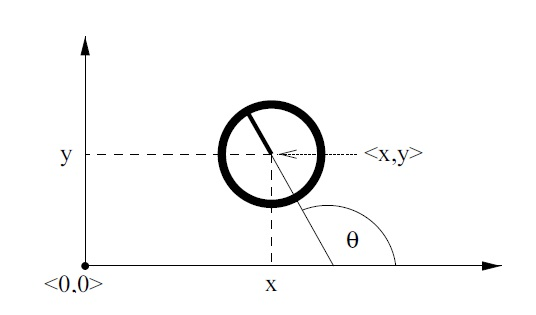
\includegraphics[width=0.9\linewidth]{51orig}}
	\caption{ (  Рис. 5.1 Положение робота в глобальной системе координат. )}
	\label{fig:51orig}
\end{figure}

Обозначив координаты через $x$ и $y$ (не следует путать с переменной состояния $x_t$), а угол - $\theta$, положение можно описать следующим вектором:\\

(5.1)
\begin{equation*}
\left(\begin{array}{c}
x\\
y\\
\theta\\
\end{array}\right)
\end{equation*}

КУРС
Угол ориентации робота часто называют \textit{курс}, или \textit{угол направления}. Как показано на Рис. 5.1, определим, что робот с курсом $\theta = 0$ направлен вдоль оси $x$. Робот, ориентированный с $\theta=0,5\pi$ указывает в направлении оси $y$.

МЕСТОПОЛОЖЕНИЕ 

Положение без учёта ориентации называется \textit{местоположением}. Концепция местоположения играет важную роль в следующей главе, посвящённой измерениям, как способу описания окружающей среды робота. Для простоты, в книге местоположения обычно будут описываться двухмерными векторами, соответствующими координатам объекта на плоскости:

(5.2)
\begin{equation*}
\left(\begin{array}{c}
x\\
y\\
\end{array}\right)
\end{equation*}

Положение робота и набор местоположений объектов окружающей среды может образовывать кинематическое состояние $x_t$ системы «робот- окружающая среда».\\

\textbf{5.2.2 Вероятностная кинематика}\\

Вероятностная кинематическая модель, или модель движения, играет в мобильной робототехнике роль модели перехода состояний. Эта модель представляет собой уже знакомую условную плотность\\

(5.3)
$$p(x_t|u_t,x_{t-1})$$ 

Здесь $x_t$ и $x_{t-1}$ – положения робота (а не просто значения его $x$-координаты), а
$u_t$ – управляющая команда на выполнение движения. Этой моделью описывается апостериорное распределение кинематических состояний, которые принимает робот при выполнении команды на движение $u_t$ в момент времени $x_{t-1}$. На практике, $u_t$ часто представлено одометрией робота. Из содержательных соображений будем, все-таки, считать $u_t$ управляющим воздействием.\\

\begin{figure}[H]
	\center{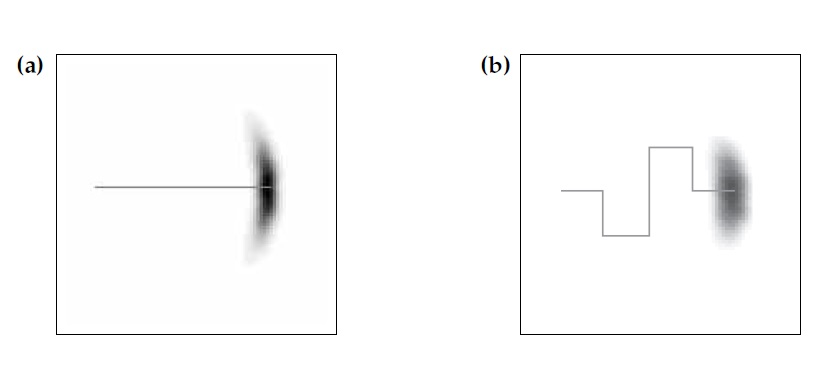
\includegraphics[width=0.9\linewidth]{52orig}}
	\caption{ (  Рис. 5.2 Модель движения: Апостериорные распределения для положения робота при выполнении команды на движение, показанной сплошной линией. Чем темнее местоположение, тем больше вероятность. График был спроектирован в 2-D. В оригинале плотность трехмерна, поскольку учитывается ещё и угол направления $\theta$ робота. )}
	\label{fig:52orig}
\end{figure}

На Рис. 5.2 показаны два примера, иллюстрирующие кинематическую модель жёсткого мобильного робота, действующего на плоскости. В обоих случаях начальное положение робота $x_{t-1}$. Распределение $p(x_t | u_t, x_{t-1})$ показано закрашенной областью: чем темнее положение, тем оно вероятнее. На рисунке вероятность апостериорного положения спроектировано на плоскость, а измерение, в котором учитывается ориентация робота, отсутствует. На Рис. 5.2a робот двигается вперёд на некоторое расстояние. Как показано на рисунке, в процессе движения могут возникнуть ошибки оценки поступательного и вращательного движения. На Рис. 5.2b показано результирующее распределение после выполнения более сложной команды на движение, что привело к большему разбросу неопределённости. 

В этой главе будут детально разобраны две отдельные вероятностные модели движения $p(x_t | u_t, x_{t-1})$ для мобильных роботов, действующих на плоскости. Обе модели взаимно по типу обрабатываемой информации о движении дополняют друг друга. В первой подразумевается, что данные о движении $u_t$ обозначают скорости вращения двигателей после подачи на них команды. Многие коммерческие мобильные роботы (с дифференциальным или синхронным приводом) независимо управляются по поступательным и вращательным скоростям, или же их лучше всего описать таким образом. Вторая модель подразумевает наличие доступа к данным одометрии. Большинство коммерческих шасси предоставляют данные одометрии, в виде кинематической информацию, например, пройденного пути и суммарного угла поворота. В результате, вероятностная модель для интеграции таких данных несколько отличается от модели скоростей. 

На практике модели одометрии часто более точны по сравнению с моделями скоростей просто в силу неспособности большинства коммерческих роботов  выполнять команды на достижение определённой скорости с той же точностью, которую можно достичь, измеряя количество оборотов колес. Однако, данные одометрии доступны только после выполнения команды на движение, и, поэтому непригодны для планирования движения. Алгоритмы планирования, такие как методы предотвращения столкновений, должны прогнозировать эффект движения. Поэтому, одометрия обычно используется для оценки, а модели скорости – для вероятностного планирования движения.\\

\textbf{5.3 Модель движения на основе скорости}\\

\textit{Модель движения на основе скорости} подразумевает, что робот управляется установкой двух скоростей, вращательной и поступательной. Множество коммерческих роботов имеют интерфейсы управления, позволяющие программистам определяет скорости. Приводные механизмы, обычно управляемые таким образом, включают дифференциальные приводы, приводы Аккермана и синхронные приводы. Модель непригодна для приводов с неголономным набором ограничений, например, колесом Илона или шагающих роботов. 

Определим поступательную скорость в момент времени $t$ через $v_t$, а \textit{вращательную скорость} - как $\omega_t$. Отсюда,\\

(5.4)
\begin{minipage}{0.1\textwidth}
	\begin{equation*}
u_t
	\end{equation*}
\end{minipage}
\begin{minipage}{0.1\textwidth}
	\begin{equation*}
	\mbox {=} \hspace{10mm} 
	\left(\begin{array}{c}
	v_t\\
\omega_t\\
	\end{array}\right)
	\end{equation*}
\end{minipage}\\

Произвольно условимся, что положительные вращательные скорости $\omega_t$ означают вращение против часовой стрелки, то есть повороты налево. Положительные поступательные скорости $v_t$ соответствуют движению вперёд.\\

\textbf{5.3.1 Вычисление в закрытом виде}\\

Возможный алгоритм вычисления вероятности $p(x_t | u_t, x_{t-1})$ показан в Таблице 5.1. На вход подаются начальное положение  $x_{t-1} = (x\, y\, \theta)^T$, управляющее воздействие $u_t = (v\, \omega)^T$ и предполагаемое последующее положение $x_t = (x'\, y'\, \theta')^T$ . На выходе возвращается вероятность $p(x_t | u_t, x_{t-1})$ нахождения системы в состоянии $x_t$ после выполнения команды $u_t$ из начального состояния $x_{t-1}$. Будем считать, что управление осуществляется в течение фиксированного промежутка времени $\varDelta t$. Серией параметров от $\alpha_1$ до $\alpha_6$ определяются конкретные виды ошибок движения. Алгоритм в Таблице 5.1 вычисляет управляющее воздействие идеального робота. Значения каждой переменной при вычислении будет описано в разделе математического вывода. Параметры заданы через $\hat{v}$
и $\hat{\omega}$.

\begin{figure}[H]
	\center{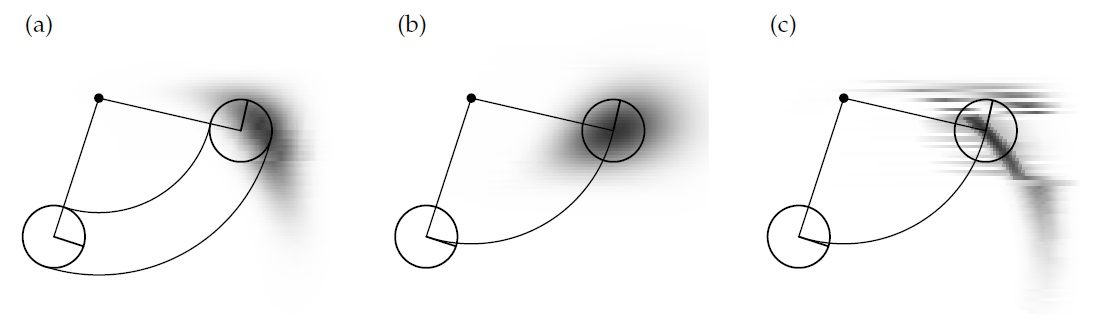
\includegraphics[width=0.9\linewidth]{53orig}}
	\caption{ (  Рис. 5.3 Модель движения на основе скорости при различных установках параметра зашумления.)}
	\label{fig:53orig}
\end{figure}

Функцией prob$(x, b^2)$ моделируется ошибка движения с помощью вычисления вероятности параметра $x$ случайной переменной с центром в нуле и дисперсией $b^2$. Две возможные реализации показаны в Таблице 5.2, где переменные ошибок представлены нормальным и треугольным распределением, соответственно. 

На Рис. 5.3 показаны примеры модели движения на основе скорости в виде проекций на плоскость. Во всех трёх случаях для робота устанавливаются одинаковые поступательные и вращательные скорости. На Рис. 5.3a показано результирующее распределение с умеренным значением параметров ошибки с $\alpha_1$ до $\alpha_6$. Распределение, показанное на Рис. 5.3b, получено с меньшей угловой ошибкой (параметры $\alpha_3$ и $\alpha_4$) но большей ошибкой поступательного движения (параметры $\alpha_1$ и $\alpha_2$). На Рис. 5.3c показано распределение с большими значениями ошибок.\\

\textbf{5.3.2 Алгоритм выборки}\\

Для многочастичных фильтров (см. подраздел 4.3) допустимо выполнять выборку из модели движения $p(x_t | u_t, x_{t-1})$ вместо вычисления апостериорного распределения произвольных $x_t$, $u_t$ и $x_{t-1}$. Взятие выборки условной плотности отличается от её вычисления набором начальных данных: При выполнении выборки даны $u_t$ и $x_{t-1}$ и необходимо сгенерировать случайное $x_t$ из выборки согласно модели движения $p(x_t | u_t, x_{t-1})$. При вычислении вероятности, кроме указанных величин, дано ещё и $x_t$, сгенерированное с помощью других значений математического ожидания, а требуется вычислить вероятность $x_t$ при $p(x_t | u_t, x_{t-1})$.

Алгоритм \textbf{sample\_motion\_model\_velocity} в Таблице 5.3 генерирует случайные элементы выборки  $p(x_t | u_t, x_{t-1})$ для фиксированного воздействия управления $u_t$ и положения $x_{t-1}$. Он принимает на вход $x_{t-1}$ и $u_t$, a генерирует случайное положение $x_t$ в соответствии с распределением $p(x_t | u_t, x_{t-1})$. В строках с 2 по 4 выполняется «искажение» параметров команды управления шумами, извлечёнными из параметров ошибки кинематической модели движения. Значения шумов затем используются для генерации нового положения, в строках с 5 по 7. 

\begin{table}[H]
\begin{center}
\begin{tabular}{|l|}
\hline
{}\\
1: \hspace{3mm} Algorithm motion\_model\_velocity $(x_t,u_t,x_{t-1}):$ \\
{}\\
2: \hspace{7mm} 
$\mu=\frac{1}{2}\,\frac{(x-x')\cos\theta+(y-y')\sin\theta}{(y-y')\cos\theta-(x-x')\sin\theta}$\\
3: \hspace{7mm} $x^*=\frac{x+x'}{2}+\mu(y-y')$\\
4: \hspace{7mm} $y^*=\frac{y+y'}{2}+\mu(x'-x)$\\
5: \hspace{7mm} $r^*=\sqrt{(x-x^*)^2+(y-y^*)^2}$\\
6: \hspace{7mm}  $\varDelta\theta=\text{atan}2(y'-y^*,x'-x^*)-\text{atan}2(y-y^*,x-x^*)$\\
7:  \hspace{8mm}$\hat{v}=\frac{\varDelta\theta}{\varDelta t}\,r^*$\\
8: \hspace{8mm}$\hat{\omega}=\frac{\varDelta\theta}{\varDelta t}$\\
9: \hspace{8mm}$\hat{\gamma}=\frac{\theta'-\theta}{\varDelta t}-\hat{\omega}$\\
10:\hspace{6mm}
\textit{return}\,$\text{prob}(v-\hat{v},\alpha_1v^2+\alpha_2\omega^2)\,\cdot\,\text{prob}(\omega-\hat{\omega},\alpha_3v^2+\alpha_4\omega^2)$\\
\hspace{21mm}$\cdot\,\text{prob}(\hat{\gamma},\alpha_5v^2+\alpha_6\omega^2)$\\
{}\\
\hline
\end{tabular}
\caption{(Таблица 5.1 Алгоритм вычисления $p(x_t | u_t, x_{t-1})$ на основании данных скорости.
Подразумевается, что $x_{t-1}$ выражено вектором $(x\,y\, \theta)^T$, $x_t$ выражено через
$(x'\,y'\,\theta')^T$, а $u_t$ - вектором скоростей $(v\,\omega)^T$. Функция prob$(a, b^2)$ вычисляет вероятность аргумента в распределении с центром в нуле и дисперсией $b^2$. Она может быть реализована на практике, используя любой из алгоритмов в Таблице 5.2.
	)}
\end{center}
\end{table}

\begin{table}[H]
\begin{center}
\begin{tabular}{|l|}
\hline
{}\\
1: \hspace{3mm} Algorithm prob\_normal\_distribution $(a,b^2):$ \\
{}\\
2:\hspace{7mm}$\textit{return}\,\frac{1}{\sqrt{2\pi \,b^2}}\,\exp\left\lbrace -\frac{1}{2}\frac{a^2}{b^2}\right\rbrace$\\
{}\\
3:\hspace{3mm} Algorithm prob\_triangular\_distribution $(a,b^2):$ \\
{}\\
4:\hspace{7mm}$\textit{return}\,\max\left\lbrace 0,\,\frac{1}{\sqrt{6}\,b}-\frac{|a|}{6\,b^2}\right\rbrace$\\ 
{}\\
\hline
\end{tabular}
\caption{(Таблица 5.2 Алгоритмы вычисления плотностей нормального и треугольного распределений с нулевым математическим ожиданием и дисперсией $b^2$.)}
\end{center}
\end{table}

\begin{table}[H]
\begin{center}
\begin{tabular}{|l|}
\hline
{}\\
1: \hspace{3mm} Algorithm sample\_motion\_model\_velocity $(u_t,x_{t-1}):$ \\
{}\\
2:\hspace{7mm}$\hat{v}=v+\text{sample}(\alpha_1v^2+\alpha_2\omega^2)$\\
3:\hspace{7mm}$\hat{\omega}=\omega+\text{sample}(\alpha_3v^2+\alpha_4\omega^2)$\\
4:\hspace{7mm}$\hat{\gamma}=\text{sample}(\alpha_5v^2+\alpha_6\omega^2)$\\
5:\hspace{7mm}$x'=x-\frac{\hat{v}}{\hat{\omega}}\sin\theta+\frac{\hat{v}}{\hat{\omega}}\sin(\theta+\hat{\omega}\varDelta t)$\\
6:\hspace{7mm}$y'=y+\frac{\hat{v}}{\hat{\omega}}\cos\theta-\frac{\hat{v}}{\hat{\omega}}\cos(\theta+\hat{\omega}\varDelta t)$\\
7:\hspace{7mm}$\theta'=\theta+\hat{\omega}\varDelta t+\hat{\gamma}\varDelta t$\\
8:\hspace{7mm}$\textit{return}\,x_t=(x',y',\theta')^T$\\ 
{}\\
\hline
\end{tabular}
\caption{(Таблица 5.3 Алгоритм выполнения выборки по положению $x_t = (x'\,y'\,\theta')^T$ из положения $x_{t-1} =
(x\,y\,\theta)^T$ и управляющего воздействия $u_t = (v\,\omega)^T$ . Обратите внимание на искажение значения конечной ориентации добавлением случайного слагаемого $\hat{\gamma}$. Переменные с $\alpha_1$ до $\alpha_6$  - параметры шумов движения. Функция sample$(b^2)$ генерирует случайный элемент выборки из распределения с нулевым математическим ожиданием и дисперсией $b^2$. Она может быть реализована, например, с помощью алгоритма в Таблице 5.4.)}
\end{center}
\end{table}

\begin{table}[H]
\begin{center}
\begin{tabular}{|l|}
\hline
{}\\
1: \hspace{3mm} Algorithm sample\_normal\_distribution $(b^2):$ \\
{}\\
2:\hspace{7mm}$\textit{return}\,\frac{1}{2}\,\sum_{i=1}^{12}\text{rand}(-b,\,b)$\\
{}\\
3:\hspace{3mm} Algorithm sample\_triangular\_distribution $(b^2):$ \\
{}\\
4:\hspace{7mm}$\textit{return}\,\frac{\sqrt{6}}{2}\,[\text{rand}(-b,\,b)+\text{rand}(-b,\,b)]$\\ 
{}\\
\hline
\end{tabular}
\caption{(Table 5.4 Алгоритм для извлечения элемента выборки из (приблизительно) нормальных и треугольных распределений с нулевым математическим ожиданием и дисперсией $b^2$. См. Винклер (Winkler, 1995: стр. 293). Функция rand$(x, y)$ считается генератором псевдослучайных чисел с однородным распределением в диапазоне $[x, y]$.)}
\end{center}
\end{table}

\begin{figure}[H]
	\center{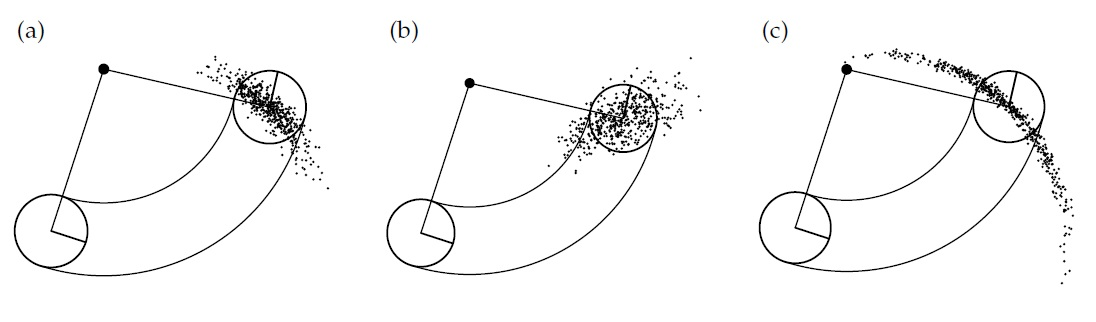
\includegraphics[width=0.9\linewidth]{54orig}}
	\caption{ (  Рис. 5.4 Выборка из модели движения на основе скоростей, используя тот же набор параметров, что и на Рис. 5.3. На каждой схеме показано 500 элементов.)}
	\label{fig:54orig}
\end{figure}

Таким образом, процедура выборки реализует упрощённую модель движения физического робота, которая учитывает шумы управления на шаге экстраполяции. На Рис. 5.4 показан итог работы последовательности выполнения выборки. На нем изображено 500 элементов выборки, сгенерированные алгоритмом sample\_motion\_model\_velocity. Читатель может самостоятельно сравнить этот рисунок с плотностью, изображённой на Рис. 5.3.

Заметим, что во многих случаях легче получить выборку $x_t$, чем высчитывать плотность вероятности для данного $x_t$. Это происходит потому, что выборка требует только прямого прохода по физической модели движения. Для вычисления вероятности предполагаемого положения необходимо восстановить параметры ошибки, что требует вычисления обратной физической модели. Факт того, что многочастичные фильтры основаны на выборке, делает их особенно привлекательными для практической реализации.\\ 

\textbf{5.3.3 Математический вывод модели движения на основе скоростей} \\

Давайте выведем алгоритмы motion\_model\_velocity и sample\_motion \_model\_velocity. Как обычно, читатель, не заинтересованный в математических подробностях, может пропустить этот раздел при первом чтении и продолжить чтение с подраздела 5.4 (страница 132???). Вывод начинается с генеративной модели движения робота, с последующим определением формул для выборки и вычисления $p(x_t | u_t, x_{t-1})$ для произвольных $x_t$, $u_t$, и $x_{t-1}$.\\

\textbf{Идеальное движение}\\

\begin{figure}[H]
	\center{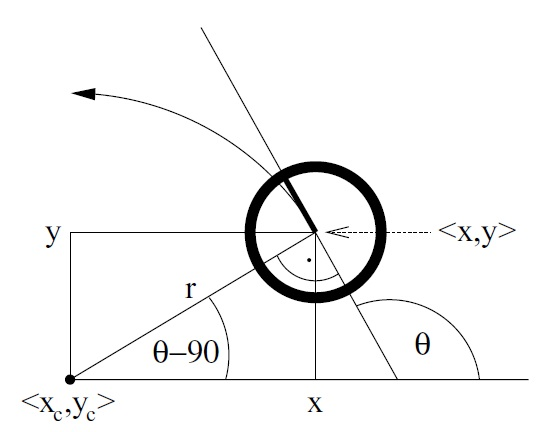
\includegraphics[width=0.9\linewidth]{55orig}}
	\caption{ (  Рис. 5.5 Движение, выполняемое роботом без зашумления, передвигающимся с постоянными скоростями 
	$v$ и $\omega$ из начальной точки $(x\,y\,\theta)^T$.)}
	\label{fig:55orig}
\end{figure}

Перед тем, как перейти к вероятностному описанию, начнём с кинематики идеального, не подверженного зашумлению робота. Пусть $u_t = (v\,\omega)^T$ определяет управляющее воздействие в момент времени $t$. Если сохраняется фиксированное значение обеих скоростей на всем интервале времени $(t-1,t)$,
робот движется по окружности радиуса\\

(5.5)
$$r=\left| \frac{v}{\omega}\right| $$

Это следует из общей взаимосвязи между поступательной и вращательной скоростями $v$ и $\omega$ для произвольного объекта, движущегося по круговой траектории с радиусом $r$:\\

(5.6)
$$v=\omega\,\cdot\,r$$

Выражение (5.5) описывает случай, когда робот не поворачивает совсем (то есть
$\omega = 0$), и движется по прямой линии. Прямая соответствует кругу бесконечного радиуса, поэтому заметим, что $r$ может быть бесконечным.

Пусть $x_{t-1} = (x,y,\theta)^T$  будет начальным положением робота, и, допустим, скорость остаётся постоянной по $(v\,\omega)^T$ в течение некоторого промежутка времени $\varDelta t$. Как легко показать, центр окружности находится в месте с координатами\\

(5.7)
$$x_c=x-\frac{v}{\omega}\sin\theta$$

(5.8)
$$y_c=y+\frac{v}{\omega}\cos\theta$$

Переменные $(xc\, yc)^T$ обозначают эти координаты. После движения в течение промежутка времени $\varDelta t$ идеальный робот будет находиться в $x_t = (x',y',\theta')^T$ с

(5.9)
\begin{minipage}{0.3\textwidth}
	\begin{equation*}
	\left(\begin{array}{c}
	x'\\
	y'\\
	\theta'\\
	\end{array}\right)
	\end{equation*}
\end{minipage}
\begin{minipage}{0.3\textwidth}
	\begin{equation*}
	\mbox {=} \hspace{10mm} 
	\left(\begin{array}{c}
	x_c+\frac{v}{\omega}\sin(\theta+\omega\varDelta t)\\
	y_c-\frac{v}{\omega}\cos(\theta+\omega\varDelta t)\\
	\theta+\omega\varDelta t\\
	\end{array}\right)
	\end{equation*}
\end{minipage}\\

\begin{minipage}{0.3\textwidth}
	\begin{equation*}
	\hspace{10mm}
	\mbox {=} \hspace{10mm}\left(\begin{array}{c}
	x\\
	y\\
	\theta\\
	\end{array}\right)
	\end{equation*}
\end{minipage}
\begin{minipage}{0.3\textwidth}
	\begin{equation*}
	\mbox {+} \hspace{2mm} 
	\left(\begin{array}{c}
	-\frac{v}{\omega}\sin\theta+\frac{v}{\omega}\sin(\theta+\omega\varDelta t)\\
	\frac{v}{\omega}\cos\theta-\frac{v}{\omega}\cos(\theta+\omega\varDelta t)\\
    \omega\varDelta t\\
	\end{array}\right)
	\end{equation*}
\end{minipage}\\

Вывод этого выражения следует из простых тригонометрических зависимостей: После
$\varDelta t$ единиц времени, идеальный робот передвинется по кругу на $v \cdot \varDelta t$, что приведёт к повороту угла направления на $\omega\cdot\varDelta t$. В то же время, его координаты $x$ и $y$ заданы пересечением окружности с центром $(x_c\,y_c)^T$ и луча, имеющего начало в $(x_c\,y_c)^T$ и перпендикулярном $\omega\cdot\varDelta t$. Во втором преобразовании в результирующие уравнения движения просто подставляется выражение (5.8).

Конечно, реальные роботы неспособны мгновенно изменять скорость и сохранять её постоянной в течение всего промежутка времени, поэтому для вычисления кинематики обычно используются малые значения $\varDelta t$, в течение которых скорость считается постоянной. Приближенное конечное положение можно получить, связывая соответствующие круговые траектории с помощью математических уравнений, которые только что были приведены.\\ 

\textbf{Реальное движение}\\

В реальности движение робота подвержено зашумлению, поэтому реальные скорости отличаются от указанных (или измеренных, если робот оснащён датчиками измерения скорости). Смоделируем это различие случайной переменной с нулевым математическим ожиданием и конечной дисперсией. Более формально, примем, что скорости заданы в виде\\

(5.10) 
\begin{minipage}{0.3\textwidth}
	\begin{equation*}
	\left(\begin{array}{c}
	\hat{v}\\
	\hat{\omega}\\
	\end{array}\right)
	\hspace{4mm}
	\mbox {=} \hspace{4mm}\left(\begin{array}{c}
	v\\
	\omega\\
	\end{array}\right)
	\end{equation*}
\end{minipage}
\begin{minipage}{0.3\textwidth}
	\begin{equation*}
	\mbox {+} \hspace{2mm} 
	\left(\begin{array}{c}
	\varepsilon_{\alpha_1v^2+\alpha_2\omega^2}\\
	\varepsilon_{\alpha_3v^2+\alpha_4\omega^2}\\
	\end{array}\right)
	\end{equation*}
\end{minipage}\\

Здесь $\varepsilon_{b^2}$ - переменная с нулевым математическим ожиданием и дисперсией $b^2$. Таким образом, реальная скорость равна сумме заданной скорости и некоторой малой, аддитивной ошибки (шумов). 
В нашей модели стандартное отклонение ошибки пропорционально заданной скорости. Параметры от $\alpha_1$ до $\alpha_4$ (где $\alpha_i\geq0$ для $i = 1, . . . , 4$) являются специфическими для робота параметрами ошибки. С их помощью моделируется точность робота, и чем она меньше, тем больше значения параметров. 

\begin{figure}[H]
	\center{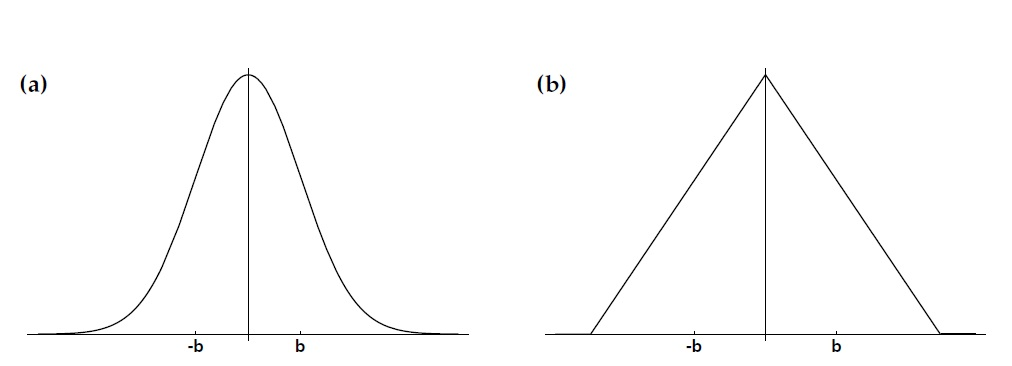
\includegraphics[width=0.9\linewidth]{56orig}}
	\caption{ (  Рис. 5.6 Функции плотности вероятности с дисперсией $b^2$: (a) Нормальное распределение,(b)треугольное распределение.)}
	\label{fig:56orig}
\end{figure}

Общепринятым способом задания ошибки $\varepsilon_{b^2}$ является использование нормального или треугольного распределений.

НОРМАЛЬНОЕ РАСПРЕДЕЛЕНИЕ
 
\textit{Нормальное распределение} с нулевым средним и дисперсией $b^2$ задано функцией плотности\\

(5.11)
$$\varepsilon_{b^2}(a)=\frac{1}{\sqrt{2\pi b^2}}e^{-\frac{1}{2}\frac{a^2}{b^2}}$$

На Рис. 5.6a показана функция плотности нормального распределения
$b^2$. Нормальные распределения обычно используются для моделирования шумов в непрерывных стохастических процессах. Её носитель, то есть набор точек a для которых $p(a) > 0$, равен $\Re$.
 
ТРЕУГОЛЬНОЕ РАСПРЕДЕЛЕНИЕ

Плотность \textit{треугольного распределения} с нулевым математическим ожиданием и дисперсией $b^2$ задана в виде\\

(5.12)
$$\varepsilon_{b^2}(a)=\max\left\lbrace 0,\frac{1}{\sqrt{6}\,b}-\frac{|a|}{6\,b^2}\right\rbrace$$ 
и не равна нулю только в промежутке $(-\sqrt{6\,b};\sqrt{6\,b})$. Как видно из Рис. 5.6b, график плотности по форме напоминает равнобедренный треугольник, отсюда и название.

Наилучшей моделью реального положения $x_t=(x'\,y'\,\theta')$ после выполнения команды на движение $u_t = (v\,\omega)^T$ в момент времени $x_{t-1} = (x\,y\,\theta)^T$, таким образом, будет \\

(5.13)
\begin{minipage}{0.3\textwidth}
	\begin{equation*}
	\left(\begin{array}{c}
	x'\\
	y'\\
	\theta'\\
	\end{array}\right)
	\hspace{2mm}
	\mbox {=} \hspace{2mm}\left(\begin{array}{c}
	x\\
	y\\
	\theta\\
	\end{array}\right)
	\end{equation*}
\end{minipage}
\begin{minipage}{0.3\textwidth}
	\begin{equation*}
	\mbox {+} \hspace{2mm} 
	\left(\begin{array}{c}
	-\frac{\hat{v}}{\hat{\omega}}\sin\theta+\frac{\hat{v}}{\hat{\omega}}\sin(\theta+\hat{\omega}\varDelta t)\\
	\frac{\hat{v}}{\hat{\omega}}\cos\theta-\frac{\hat{v}}{\hat{\omega}}\cos(\theta+\hat{\omega}\varDelta t)\\
	\hat{\omega}\varDelta t\\
	\end{array}\right)
	\end{equation*}
\end{minipage}\\

Это равенство получено заменой указанной скорости $u_t = (v\,\omega)^T$ зашумленным движением $(\hat{v}\,\hat{\omega})^T$ в выражении (5.9). Однако, модель все ещё не слишком реалистична в силу описанных ниже причин.\\

\textbf{Конечная ориентация}\\

Два приведённых выше равенства точно описывают конечное местоположение робота при условии, что робот движется по строго круговой траектории радиуса $r=\frac{\hat{v}}{\hat{\omega}}$ . Хотя значения радиуса этого сегмента окружности и пройденное расстояние подвержены шумам управления, сам факт движения по круговой траектории остаётся в силе. Допущение о том, что траектория является круговой, ведёт к важному преобразованию вырождения. В частности, носитель функции плотности $p(x_t | u_t, x_{t-1})$ является двухмерным, при этом находится внутри трехмерного пространства состояний. Факт нахождения всех апостериорных положений в двухмерном множестве трехмерного пространства положений является прямым следствием того факта, что было использовано только две переменных зашумления, одна для $v$ и одна - для $\omega$. К сожалению, это вырождение имеет важные последствия при использовании байесовских фильтров для оценки состояния. 

Конечно, в реальности любое осмысленное апостериорное распределение не будет вырожденным и положения будут расположены в трехмерном пространстве с дисперсией по $x, y$ и $\theta$. Чтобы соответствующим образом обобщить рассматриваемую модель, допустим, что робот выполняет поворот $\hat{\gamma}$, когда достигает конечного положения. Поэтому, вместо вычисления $\theta'$ в соответствии с (5.13), смоделируем конечную ориентацию \\

(5.14)
$$\theta'=\theta+\hat{\omega}\varDelta t+\hat{\gamma}\varDelta t$$

c\\

(5.15)
$$\hat{\gamma}=\varepsilon_{\alpha_5v^2+\alpha_6\omega^2}$$

Здесь $\alpha_5$ и $\alpha_6$ – дополнительные параметры робота, определяющие дисперсию добавочного зашумления вращения. Результирующая модель будет выглядеть следующим образом:\\

(5.16) 
\begin{minipage}{0.3\textwidth}
	\begin{equation*}
	\left(\begin{array}{c}
	x'\\
	y'\\
	\theta'\\
	\end{array}\right)
	\hspace{2mm}
	\mbox {=} \hspace{2mm}\left(\begin{array}{c}
	x\\
	y\\
	\theta\\
	\end{array}\right)
	\end{equation*}
\end{minipage}
\begin{minipage}{0.3\textwidth}
	\begin{equation*}
	\mbox {+} \hspace{2mm} 
	\left(\begin{array}{c}
	-\frac{\hat{v}}{\hat{\omega}}\sin\theta+\frac{\hat{v}}{\hat{\omega}}\sin(\theta+\hat{\omega}\varDelta t)\\
	\frac{\hat{v}}{\hat{\omega}}\cos\theta-\frac{\hat{v}}{\hat{\omega}}\cos(\theta+\hat{\omega}\varDelta t)\\
	\hat{\omega}\varDelta t+\hat{\gamma}\varDelta t\\
	\end{array}\right)
	\end{equation*}
\end{minipage}\\

\textbf{Вычисление $p(x_t | u_t, x_{t-1})$}\\

Алгоритм \textbf{motion\_model\_velocity} в Таблице 5.1 реализует вычисление $p(x_t | u_t, x_{t-1})$ для заданных значений $x_{t-1} = (x\,y\,\theta)^T$ , $u_t = (v\,\omega)^T$ , и $x_t = (x\,y\,\theta)^T$. Вывод алгоритма несколько неочевиден, поскольку в нем эффективно реализуется обратная модель движения. В частности, motion\_model \_velocity на основании положений $x_{t-1}$ и $x_t$ определяет параметры движения $\hat{u}_t=(\hat{v}\,\hat{\omega})^T$ а также соответствующий конечный поворот $\hat{\gamma}$. Вывод очевидно доказывает необходимость конечного поворота, поскольку без него вероятность движения почти для всех значений $x_{t-1}$, $u_t$, и $x_t$, будет равна нулю. 

Давайте вычислим вероятность $p(x_t | u_t, x_{t-1})$ действия управления $u_t = (v\,\omega)^T$,
которое перенесёт робота из положения $x_{t-1} = (x\,y\,\theta)^T$ в положение $x_t = (x'\,y'\,\theta')^T$
в течение времени $\varDelta t$. Чтобы это сделать, определим управляющее воздействие $\hat{u}=(\hat{v}\,\hat{\omega})^T$, требуемое для переноса робота из положения $x_{t-1}$ в положение $(x'\,y')$ безотносительно конечного угла направления. Далее, станет возможным определить конечный поворот 
$\hat{\gamma}$, который необходимо выполнить роботу для перехода к углу направления $\theta'$. На основании этих вычислений легко найти вероятность $p(x_t | u_t, x_{t-1})$.

Читатель может вспомнить, что в нашей модели подразумевалось перемещение робота с фиксированной скоростью по круговой траектории в течение времени $\varDelta t$. Для робота, который переместился из $x_{t-1} = (x\,y\,\theta)^T$ к $x_t = (x'\,y')^T$, центр окружности будет определён как $(x^*\,y^*)^T$ и задан в виде\\

(5.17)
\begin{minipage}{0.3\textwidth}
	\begin{equation*}
	\left(\begin{array}{c}
	x^*\\
	y^*\\
	\end{array}\right)
	\hspace{2mm}
	\mbox {=} \hspace{2mm}\left(\begin{array}{c}
	x\\
	y\\
	\end{array}\right)
	\end{equation*}
\end{minipage}
\begin{minipage}{0.3\textwidth}
	\begin{equation*}
	\mbox {+} \hspace{2mm} 
	\left(\begin{array}{c}
	-\lambda\sin\theta\\
	\lambda\cos\theta\\
	\end{array}\right)
	\hspace{2mm}
	\mbox {=} \hspace{2mm}\left(\begin{array}{c}
	\frac{x+x'}{2}+\mu(y-y')\\
	\frac{y+y'}{2}+\mu(x'-x)\\
	\end{array}\right)
	\end{equation*}
\end{minipage}\\

для некоторых неизвестных $\lambda,\mu\in\Re$. Первое равенство стало результатом ортогональности направления на центр окружности первоначальному углу направления робота. Второе является очевидным заключением о том, что центр окружности лежит на прямой, которая пролегает посередине между
$(x\,y)^T$ и $(x'\,y')^T$ и ортогональна соединяющей их прямой.

Обычно, выражение (5.17) имеет единственное решение, за исключением вырожденного случая, когда $\omega=0$, а центр окружности находится в бесконечности. Как читатель может захотеть проверить,\\

(5.18)
$$\mu=\frac{1}{2}\frac{(x-x')\cos\theta+(y-y')\sin\theta}{(y-y')\cos\theta-(x-x')\sin\theta}$$

поэтому\\

(5.19)
\begin{minipage}{0.2\textwidth}
	\begin{equation*}
	\left(\begin{array}{c}
	x^*\\
	y^*\\
	\end{array}\right)
	\end{equation*}
\end{minipage}
\begin{minipage}{0.2\textwidth}
	\begin{equation*}
	\mbox {=} \hspace{5mm}
	\left(\begin{array}{c}
	\frac{x+x'}{2}+\frac{1}{2}\frac{(x-x')\cos\theta+(y-y')\sin\theta}{(y-y')\cos\theta-(x-x')\sin\theta}(y-y')\\
	\frac{y+y'}{2}+\frac{1}{2}\frac{(x-x')\cos\theta+(y-y')\sin\theta}{(y-y')\cos\theta-(x-x')\sin\theta}(x'-x)\\
	\end{array}\right)
	\end{equation*}
\end{minipage}\\

радиус окружности задан евклидовым расстоянием\\

(5.20)
$$r^*=\sqrt{(x-x^*)^2+(y-y^*)^2}=\sqrt{(x'-x^*)^2+(y'-y^*)^2}$$

Теперь стало возможным вычислить изменение угла направления\\

(5.21)
$$\varDelta\theta=\text{atan}2(y'-y^*,x'-x^*)-\text{atan}2(y-y^*,x-x^*)$$

Здесь atan2 это широко известное расширение арктангенса $y/x$, расширенного до $\Re^2$ (в большинстве языков программирования есть реализация этой функции):\\

(5.22)
\begin{equation*}
\text{atan}2(y,x)=\left\{
\begin{array}{ll}
\text{atan}(y/x) & \mbox{ если }x>0\\
\text{sign}(y)(\pi-\text{atan}(|y/x|))& \mbox{ если }x<0\\
0&\mbox{ если }x=y=0\\
\text{sign}(y)\pi/2& \mbox{ если }x=0,y\neq0\\
\end{array}
\right.
\end{equation*}

Поскольку было принято, что робот движется по круговой траектории, расстояние между $x_t$ и $x_{t-1}$ по дуге равно\\

(5.23)
$$\varDelta\text{dist}=r^*\,\cdot\,\varDelta\theta$$

Из $\varDelta\text{dist}$ и $\varDelta\theta$ легко вычислить скорости $\hat{v}$ и $\hat{\omega}$:\\

(5.24)
\begin{minipage}{0.3\textwidth}
	\begin{equation*}
	\hspace{10mm}
	\hat{u}_t \hspace{5mm}
	\mbox{=}
	\hspace{5mm}
	\left(\begin{array}{c}
	\hat{v}\\
	\hat{\omega}\\
	\end{array}\right)
	\hspace{5mm}
	\mbox{=}
	\hspace{5mm}
	\varDelta t^{-1}
	\left(\begin{array}{c}
	\varDelta\text{dist}\\
	\varDelta\theta\\
	\end{array}\right)
	\end{equation*}
\end{minipage}\\

Скорость вращения $\hat{\gamma}$, необходимая для достижения конечного угла направления $\theta'$ робота в координатах $(x'\,y')$ за время $\varDelta t$ можно определить из (5.14) как:\\

(5.25)
$$\hat{\gamma}=\varDelta t^{-1}(\theta'-\theta)-\hat{\omega}$$

Ошибка движения - это отклонение от указанных скоростей по $\hat{u}_t$ и $\hat{\gamma}$ 
$u_t = (v\,\omega)^T$ и $\gamma=0$, как было определено выражениями (5.24) и (5.25).\\

(5.26)
$$v_{\text{err}}=v-\hat{v}$$

(5.27)
$$\omega_{\text{err}}=\omega-\hat{\omega}$$

(5.28)
$$\gamma_{\text{err}}=\hat{\gamma}$$

В нашей модели ошибок, определённой выражениями (5.10) и (5.15), эти ошибки имеют следующие вероятности:\\

(5.29)
$$\varepsilon_{\alpha_1v^2+\alpha_2\omega^2}(v_{\text{err}})$$

(5.30)
$$\varepsilon_{\alpha_3v^2+\alpha_4\omega^2}(\omega_{\text{err}})$$

(5.31)
$$\varepsilon_{\alpha_5v^2+\alpha_6\omega^2}(\gamma_{\text{err}})$$

где $\varepsilon_{b^2}$, как и прежде, означает переменную ошибки с нулевым математическим ожиданием и дисперсией $b^2$.
Поскольку подразумевается независимость между разными источниками ошибки, искомая вероятность $p(x_t | u_t, x_{t-1})$ является произведением отдельных ошибок:\\

(5.32)
$$p(x_t|u_t,x_{t-1})=\varepsilon_{\alpha_1v^2+\alpha_2\omega^2}(v_{\text{err}})\,\cdot\,\varepsilon_{\alpha_3v^2+\alpha_4\omega^2}(\omega_{\text{err}})\,\cdot\,\varepsilon_{\alpha_5v^2+\alpha_6\omega^2}(\gamma_{\text{err}})$$

Чтобы убедиться в корректности алгоритма \textbf{motion\_model\_velocity} в Таблице 5.1,
читатель может заметить, что в алгоритме реализовано именно это выражение. А именно, содержание строк со 2 по 9 эквивалентно выражениям (5.18), (5.19), (5.20), (5.21), (5.24), и (5.25). В строке 10 реализуется преобразование (5.32), заменяя выражения для ошибки, как указано в (5.29) до (5.31).\\

\textbf{Выборка из $p(x' | u, x)$}\\

Алгоритм выборки \textbf{sample\_motion\_model\_velocity} в Таблице 5.3 реализует прямую модель, описанную ранее в этом разделе. Строки с 5 по 7 соответствуют выражению (5.16). Зашумленные значения, вычисленные в строках со 2 по 4, соответствуют выражениям (5.10) и (5.15).

Алгоритм \textbf{sample\_normal\_distribution} в Таблице 5.4 реализует общий подход к выполнению выборки из нормального распределения. Это приближение использует центральную предельную теорему, которая утверждает, что любое среднее невырожденной случайной переменной сводится до нормального распределения. Путём усреднения 12 однородных распределений в алгоритме \textbf{sample\_normal\_distribution}
генерируются значения с, примерно, нормальным распределением. Технически, результирующие значения будут всегда лежать в промежутке $[-2b,2b]$. Наконец, в  \textbf{sample\_triangular\_distribution} в Таблице 5.4 реализуется выборка из множества для треугольных распределений.\\

\textbf{5.4 Модель движения на основе одометрии}\\

Модель движения на основе скорости, обсуждаемая выше, использует значения скорости робота для вычисления апостериорных распределений положений. В качестве альтернативного варианта для вычисления движения робота возможно использовать измерения одометрии. Данные одометрии обычно получаются путем интегрирования информации с энкодеров на колесах. Большинство коммерческих роботов выдают такие оценки положения через определённые интервалы времени (например, 10 раз в секунду). Это приводит к методу определения другой модели движения, обсуждаемой в этом главе – модели на основе одометрии. В ней вместо данных управления используется одометрия. 

\begin{figure}[H]
	\center{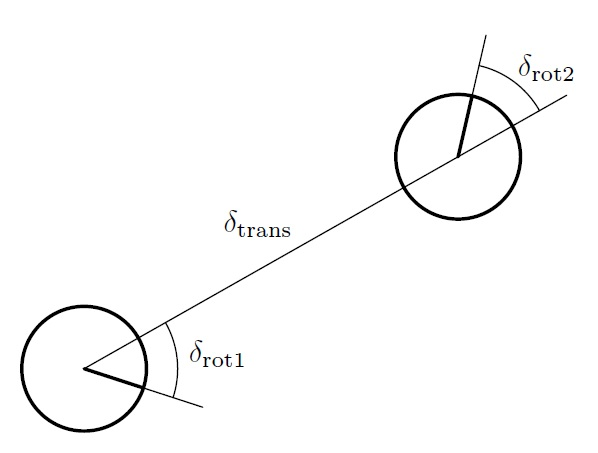
\includegraphics[width=0.7\linewidth]{57orig}}
	\caption{ (  Рис. 5.7 Модель одометрии: Робот движется в интервале времени $\left( t - 1, t\right] $ по пути, приблизительно определённом вращением $\delta_{\text{rot}1}$, перемещением $\delta_{\text{trans}}$ и вторым вращением
	$\delta_{\text{rot}2}$. Повороты и перемещения зашумлены.)}
	\label{fig:57orig}
\end{figure}

Практический опыт показывает, что одометрия, даже при наличии ошибок, обычно даёт более точные данные, чем скорость. Точность обоих показателей падает из-за пробуксовки и скольжения, но скорость, вдобавок, подвержена ещё и несоответствиям между реальными контроллерами движения и их (грубой) математической моделью. Кроме этого, данные одометрии доступны только в ретроспективе, после окончания перемещения робота. Это не является проблемой для алгоритмов фильтров, таких, как методы локализации и построения карт, обсуждаемых в следующих главах. Однако, это делает данные одометрии недоступными для задач точного планирования движения и управления.\\

\textbf{5.4.1 Вычисление в закрытом виде}\\

Технически, данные одометрии представляют собой измерения датчиков, а не управление, но при их моделировании в виде измерений результирующий байесовский фильтр должен включать текущие скорости в виде переменных состояния, что увеличивает размерность пространства состояний. Для сохранения малого размера пространства состояний, общепринято считать данные одометрии сигналами управления, поэтому и в книге будем рассматривать измерения одометров как управляющие воздействия. Результирующая модель входит в состав ядер многих лучших современных вероятностных робототехнических систем. 

Определим формат информации управления. В момент времени $t$, верное положение робота моделируется случайной переменной $x_t$. Одометрия робота является оценкой положения, но, из-за пробуксовки и проскальзывания, точный метод перевода координат между внутренней одометрией робота и координатами физического мира отсутствует. Фактически, знание такого преобразования может решить задачу локализации робота! 

В модели на основе одометрии используются относительные данные движения, измеренные внутренним одометром робота. В течение интервала времени $\left( t - 1, t\right] $,
робот перемещается из положения $x_{t-1}$ в положение $x_t$. Одометр сообщает показания относительного перемещения из $\bar{x}_{t-1}=(\bar{x}\,\bar{y}\,\bar{\theta})^T$ в $\bar{x}_t=(\bar{x}'\,\bar{y}'\,\bar{\theta}')^T$ . Здесь черта над переменной указывает на то, что измерения одометрии внесены во внутреннюю систему координат робота с неизвестным отношением к глобальной мировой системе координат .\\

\begin{table}[H]
\begin{center}
\begin{tabular}{|l|}
\hline
{}\\
1: \hspace{3mm} Algorithm motion\_model\_odometry $(x_t,u_t,x_{t-1}):$ \\
2:\hspace{7mm}$\delta_{\text{rot}1}=\text{atan}2(\bar{y}'-\bar{y},\bar{x}'-\bar{x})-\bar{\theta}$\\
3:\hspace{7mm}$\delta_{\text{trans}}=\sqrt{(\bar{x}-\bar{x}')^2+(\bar{y}-\bar{y}')^2}$\\
4:\hspace{7mm}$\delta_{\text{rot}2}=\bar{\theta}'-\bar{\theta}-\delta_{\text{rot}1}$\\
{}\\
5:\hspace{7mm}$\hat{\delta}_{\text{rot}1}=\text{atan}2(y'-y,x'-x)-\theta$\\
6:\hspace{7mm}$\hat{\delta}_{\text{trans}}=\sqrt{(x-x')^2+(y-y')^2}$\\
7:\hspace{7mm}$\hat{\delta}_{\text{rot}2}=\theta'-\theta-\hat{\delta}_{\text{rot}1}$\\
{}\\
8:\hspace{7mm}$p_1=\text{prob}(\delta_{\text{rot}1}-\hat{\delta}_{\text{rot}1},\alpha_1\hat{\delta}_{\text{rot}1}^2+\alpha_2\hat{\delta}_{\text{trans}}^2)$\\
9:\hspace{7mm}$p_2=\text{prob}(\delta_{\text{trans}}-\hat{\delta}_{\text{trans}},\alpha_3\hat{\delta}_{\text{trans}}^2+\alpha_4\hat{\delta}_{\text{rot}1}^2+\alpha_4\hat{\delta}_{\text{rot}2}^2)$\\
10:\hspace{5mm}$p_3=\text{prob}(\delta_{\text{rot}2}-\hat{\delta}_{\text{rot}2},\alpha_1\hat{\delta}_{\text{rot}2}^2+\alpha_2\hat{\delta}_{\text{trans}}^2)$\\
{}\\
11:\hspace{5mm}$\textit{return}\, p_1\,\cdot\,p_2\,\cdot\,p_3$\\
{}\\
\hline
\end{tabular}
\caption{(Таблица 5.5 Алгоритм для вычисления $p(x_t | u_t, x_{t-1})$ на основе данных одометрии.
Здесь управление $u_t$  задано в виде $(\bar{x}_{t-1}\,\bar{x}_t)^T$, с $\bar{x}_{t-1}=(\bar{x}\,\bar{y}\,\bar{\theta})$ и $\bar{x}_t=(\bar{x}'\,\bar{y}'\,\bar{\theta}')$.)}
\end{center}
\end{table}

Ключевой момент использования этой информации при оценке состояния состоит в том, что относительная разница между $\bar{x}_{t-1}$ и $\bar{x}_t$, при соответствующем определении термина, является хорошей функцией для оценки разницы реальных положений $x_{t-1}$ и $x_t$. Информация о движении $u_t$ задана в виде 

(5.33)
\begin{minipage}{0.3\textwidth}
	\begin{equation*}
	\hspace{10mm}
	u_t \hspace{5mm}
	\mbox{=}
	\hspace{5mm}
	\left(\begin{array}{c}
	\bar{x}_{t-1}\\
	\bar{x}_t\\
	\end{array}\right)
	\end{equation*}
\end{minipage}\\
Чтобы извлечь относительные данные одометрии $u_t$ необходимо выполнить преобразование для трёх последовательных этапов:
вращения, за которым следует движение по прямой линии (поступательное), и ещё одного вращения. На Рис. 5.7 это показано следующим образом: первоначальный поворот назван $\delta_{\text{rot}1}$, поступательное движение обозначено как $\delta_{\text{trans}}$, а второй поворот - $\delta_{\text{rot}2}$. Как читатель может легко убедиться, для каждой пары положений  $(\bar{s}\,\bar{s}')$ имеется уникальный вектор параметров $(\delta_{\text{rot}1}\,\delta_{\text{trans}}\,\delta_{\text{rot}2})^T$, и этих параметров достаточно для реконструкции
относительного перемещения между $\bar{s}$ и $\bar{s}'$. Таким образом, $\delta_{\text{rot}1}, \delta_{\text{trans}}, \delta_{\text{rot}2}$ образуют достаточные статистические показатели относительного движения, закодированного в виде одометрии.

\begin{figure}[H]
	\center{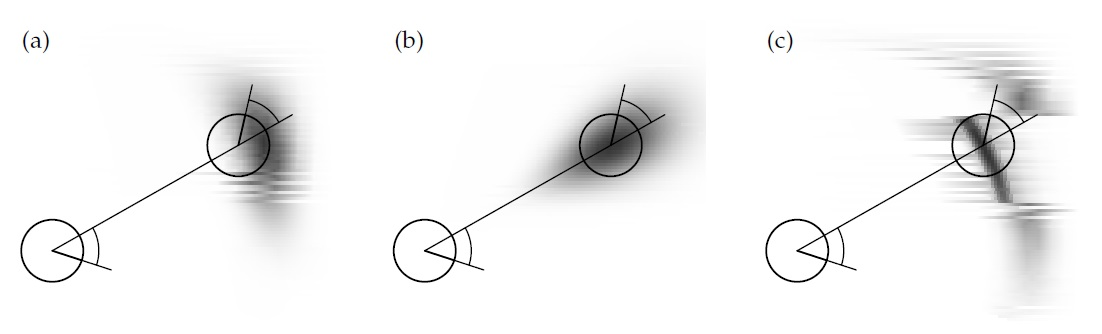
\includegraphics[width=1\linewidth]{58orig}}
	\caption{ (  Рис. 5.8 Модель движения на основе одометрии при различных значениях параметров зашумления.)}
	\label{fig:58orig}
\end{figure}

Вероятностная модель движения предполагает искажение этих трёх параметров независимыми шумами. Читатель может заметить, что при описании движения на основе одометрии используется на один параметр больше, чем в векторе скорости, определённом в предыдущем разделе. Поэтому вырождение, из-за которого мы были вынуждены использовать метод «последнего поворота», отсутствует. 

Перед тем, как погрузиться в математические подробности, определим базовый метод вычисления этой плотности в закрытом виде. В Таблице 5.5 приведён алгоритм вычисления $p(x_t | u_t, x_{t-1})$ из данных одометрии. Он принимает на вход данные о начальном положении $x_{t-1}$, пару положений $u_t = (\bar{x}_{t-1}\, \bar{x}_t)^T$, полученных из одометрии робота, и гипотетическое конечное положение $x_t$. На выход возвращается числовая вероятность $p(x_t | u_t, x_{t-1})$.

В строках со 2 по 4 в Таблице 5.5 из показаний одометрии восстанавливаются параметры относительного перемещения $(\delta_{\text{rot}1}\,\delta_{\text{trans}}\,\delta_{\text{rot}2})^T$. Как и прежде, используется \textit{обратная модель движения}. Соответствующие параметры относительного перемещения $(\hat{\delta}_{\text{rot}1}\,\hat{\delta}_{\text{trans}}\,\hat{\delta}_{\text{rot}2})^T$ для заданных положений $x_{t-1}$ и $x_t$ вычисляются в строках с 5 по 7 алгоритма. В строках с 8 по 10 вычисляются вероятности ошибок для отдельных параметров движения. Как и прежде, функция prob $(a, b^2)$ реализует распределение ошибок по $a$ с нулевым математическим ожиданием и дисперсией $b^2$. При реализации алгоритма необходимо следить, чтобы все угловые разницы находились в диапазоне $[-\pi,\pi]$. В силу этого результат $\delta_{\text{rot}2}-\bar{\delta}_{\text{rot}2}$ следует соответствующим образом сокращать — распространённая ошибка реализации, которую трудно обнаружить. Наконец, в строке 11 возвращается вероятность комбинированной ошибки, полученная перемножением отдельных вероятностей ошибки $p_1, p_2$ и $p_3$. На этом шаге подразумевается независимость различных источников ошибок. Переменные от $\alpha_1$ до $\alpha_4$ – специфические параметры робота, определяющие шумы движения.

\begin{table}[H]
\begin{center}
\begin{tabular}{|l|}
\hline
{}\\
1: \hspace{3mm} Algorithm sample\_motion\_model\_odometry $(u_t,x_{t-1}):$ \\
2:\hspace{7mm}$\delta_{\text{rot}1}=\text{atan}2(\bar{y}'-\bar{y},\bar{x}'-\bar{x})-\bar{\theta}$\\
3:\hspace{7mm}$\delta_{\text{trans}}=\sqrt{(\bar{x}-\bar{x}')^2+(\bar{y}-\bar{y}')^2}$\\
4:\hspace{7mm}$\delta_{\text{rot}2}=\bar{\theta}'-\bar{\theta}-\delta_{\text{rot}1}$\\
{}\\
5:\hspace{7mm}$\hat{\delta}_{\text{rot}1}=\delta_{\text{rot}1}-\text{sample}(\alpha_1\delta_{\text{rot}1}^2+\alpha_2\delta_{\text{trans}}^2)$\\
6:\hspace{7mm}$\hat{\delta}_{\text{trans}}=\delta_{\text{trans}}-\text{sample}(\alpha_3\delta_{\text{trans}}^2+\alpha_4\delta_{\text{rot}1}^2+\alpha_4\delta_{\text{rot}2}^2)$\\
7:\hspace{7mm}$\hat{\delta}_{\text{rot}2}=\delta_{\text{rot}2}-\text{sample}(\alpha_1\delta_{\text{rot}2}^2+\alpha_2\delta_{\text{trans}}^2)$\\
{}\\
8:\hspace{7mm}$x'=x+\hat{\delta}_{\text{trans}}\cos(\theta+\hat{\delta}_{\text{rot}1})$\\
9:\hspace{7mm}$y'=y+\hat{\delta}_{\text{trans}}\sin(\theta+\hat{\delta}_{\text{rot}1})$\\
10:\hspace{5mm}$\theta'=\theta+\hat{\delta}_{\text{rot}1}+\hat{\delta}_{\text{rot}2}$\\
{}\\
11:\hspace{5mm}$\textit{return}\,x_t=(x',y',\theta')^T$\\
{}\\
\hline
\end{tabular}
\caption{(Таблица 5.6 Алгоритм выборки из $p(x_t | u_t, x_{t-1})$ на основе данных одометрии. Здесь положение в момент времени $t$ представлено в виде $x_{t-1} = (x\,y\,\theta)^T$. Управление представляет собой дифференцируемый набор двух оценок положения, полученных одометром робота, $u_t = (\bar{x}_{t-1}\,\bar{x}_t)^T$ , где $\bar{x}_{t-1}=(\bar{x}\,\bar{y}\,\bar{\theta})$ , а $\bar{x}_t=(\bar{x}'\,\bar{y}'\,\bar{\theta}')$ .)}
\end{center}
\end{table}

На Рис. 5.8 показаны примеры модели движения на основе одометрии для разных значений параметров ошибки от $\alpha_1$ до $\alpha_4$. Если распределение на Рис. 5.8a выглядит знакомо, то на Рис. 5.8b и 5.8c показаны необычно большие ошибки перемещения и вращения. Читатель может самостоятельно сравнить эти схемы с приведёнными на Рис. 5.3 на странице 122(????). Чем меньше время между двумя последовательными измерениями, тем более схожи между собой эти две модели движения. Поэтому, если оценка обновляется достаточно часто, например 10 раз в секунду для робота, действующего внутри помещений, разница между моделями движения не слишком существенна.\\

\begin{figure}[H]
	\center{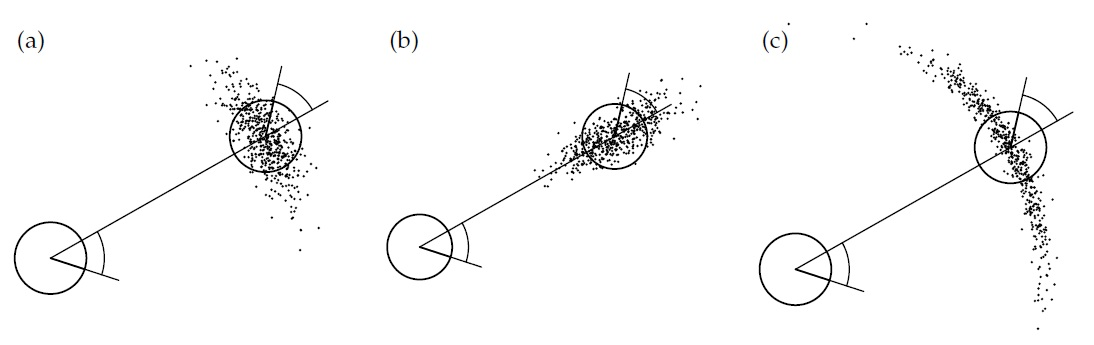
\includegraphics[width=1\linewidth]{59orig}}
	\caption{ (  Рис. 5.9 Выборка из модели движения на основе одометрии, используя те же параметры, что на Рис. 5.8. На каждой схеме показаны 500 элементов выборки.)}
	\label{fig:59orig}
\end{figure}

\textbf{5.4.2 Алгоритм выборки}\\

При использовании многочастичных фильтров в задаче локализации было бы желательно получить алгоритм  выборки из $p(x_t | u_t, x_{t-1})$. Напомним, что многочастичные фильтры (подраздел 4.3) для любых $x_{t-1}$, $u_t$ и $x_t$ требуют элементов выборки из $p(x_t | u_t, x_{t-1})$, а не выражения для вычисления в закрытой виде $p(x_t | u_t, x_{t-1})$ . Алгоритм \textbf{sample\_motion\_model\_odometry}, показанный на Рис. 5.6, реализует метод выполнения выборки. На вход принимается начальное положение $x_{t-1}$ и показания одометрии $u_t$, а на выход возвращается случайная переменная $x_t$, распределенная согласно $p(x_t | u_t, x_{t-1})$.
Отличие от предыдущего алгоритма состоит в том, что вместо вычисления вероятности данного $x_t$, случайным образом выбирается гипотеза относительно положения $x_t$ (строки 5-10). Как и прежде,
алгоритм выборки \textbf{sample\_motion\_model\_odometry} несколько проще в реализации, чем алгоритм в закрытом виде \textbf{motion\_model\_odometry}, поскольку он обходит необходимость в обратной модели.

На Рис. 5.9 показаны примеры наборов элементов выборки алгоритма \textbf{sample\_motion\_model\_odometry}, с использованием тех же параметров, что и для показанной на Рис.5.8 модели. На Рис. 5.10 показано применение модели движения с наложением выборок нескольких тактов времени. Эти данные были сгенерированы с использованием уравнений обновления движения алгоритма \textbf{particle\_filter}
(Таблица 4.3). На рисунке одометрия пути робота показана сплошной линией. Кроме того, явно виден рост неопределённости при движении робота, в результате чего выборка распределена по все более возрастающей площади.\\

\textbf{5.4.3 Математический вывод модели движения на основе одометрии}\\ 

Вывод алгоритмов довольно прямолинеен, и может быть пропущен при первом чтении. Для вывода вероятностной модели движения с использованием одометрии вспомним, что относительная разница между двумя положениями отображена суммой трёх основных движений: поворота, движения по прямой линии (поступательного), и ещё одного поворота. Следующие уравнения демонстрируют способ вычисления значений двух поворотов и поступательного движения на основе показаний одометрии $u_t=(\bar{x}_{t-1}\,\bar{x}_t)^T$, где $\bar{x}_{t-1}=(\bar{x}\,\bar{y}\,\bar{\theta})$, а $\bar{x}_t=(\bar{x}'\,\bar{y}'\,\bar{\theta}')$:\\

(5.34)
$$\delta_{\text{rot}1}=\text{atan}2(\bar{y}'-\bar{y},\bar{x}'-\bar{x})-\bar{\theta}$$

(5.35)
$$\delta_{\text{trans}}=\sqrt{(\bar{x}-\bar{x}')^2+(\bar{y}-\bar{y}')^2}$$

(5.36)
$$\delta_{\text{rot}2}=\bar{\theta}'-\bar{\theta}-\delta_{\text{rot}1}$$

\begin{figure}[H]
	\center{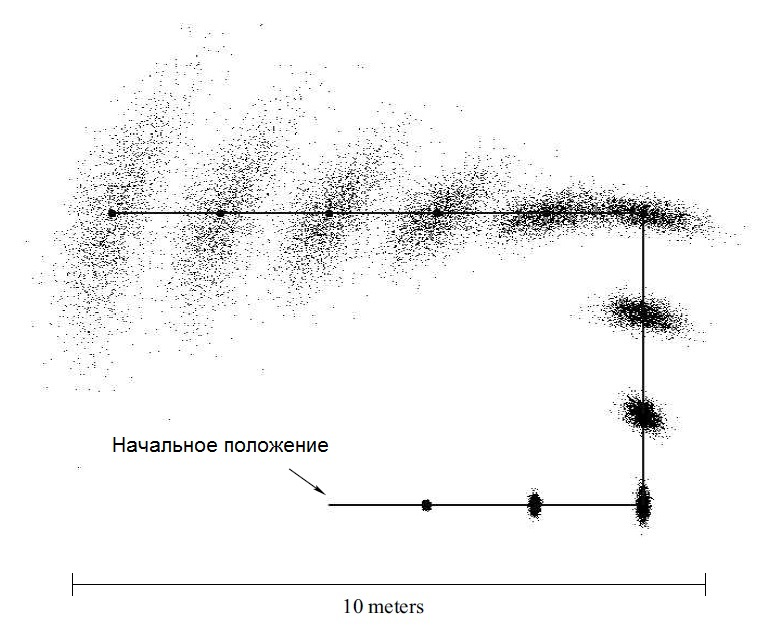
\includegraphics[width=1\linewidth]{510orig}}
	\caption{ (  Рис. 5.10 Аппроксимация выборки гипотезы местоположения для робота без датчиков. 
	Сплошной линией показаны действия, а элементы выборки отображают  относительные  местоположения робота в различные моменты времени.
		)}
	\label{fig:510orig}
\end{figure}

Для моделирования ошибки движения, допустим, что «истинные» значения поворота и поступательного движения получены из измеренных путём вычитания независимого шума $\varepsilon_{b^2}$ с нулевым математическим ожиданием и дисперсией $b^2$:\\

(5.37)
$$\hat{\delta}_{\text{rot}1}=\delta_{\text{rot}1}-\varepsilon_{\alpha_1\delta_{\text{rot}1}^2+\alpha_2\delta_{\text{trans}}^2}$$

(5.38)
$$\hat{\delta}_{\text{trans}}=\delta_{\text{trans}}-\varepsilon_{\alpha_3\delta_{\text{trans}}^2+\alpha_4\delta_{\text{rot}1}^2+\alpha_4\delta_{\text{rot}2}^2}$$

(5.39)
$$\hat{\delta}_{\text{rot}2}=\delta_{\text{rot}2}-\varepsilon_{\alpha_1\delta_{\text{rot}2}^2+\alpha_2\delta_{\text{trans}}^2}$$

Как и в предыдущем разделе, $\varepsilon_{b^2}$ - переменная зашумления с нулевым математическим ожиданием и дисперсией $b^2$.
Параметры от $\alpha_1$ до $\alpha_2$ являются специфическими параметрами ошибки робота, определяющими ошибку движения.

Следовательно, истинное местоположение $x_t$, получается из $x_{t-1}$ путём первого поворота на угол $\hat{\delta}_{\text{rot}1}$, последующего линейного движения $\hat{\delta}_{\text{trans}}$, и второго поворота на угол $\hat{\delta}_{\text{rot}2}$. Таким образом,\\

(5.40)
\begin{minipage}{0.3\textwidth}
	\begin{equation*}
	\left(\begin{array}{c}
	x'\\
	y'\\
	\theta'\\
	\end{array}\right)
	\hspace{2mm}
	\mbox {=} \hspace{2mm}\left(\begin{array}{c}
	x\\
	y\\
	\theta\\
	\end{array}\right)
	\end{equation*}
\end{minipage}
\begin{minipage}{0.3\textwidth}
	\begin{equation*}
	\mbox {+} \hspace{2mm} 
	\left(\begin{array}{c}
	\hat{\delta}_{\text{trans}}\,\cos(\theta+\hat{\delta}_{\text{rot}1})\\
	\hat{\delta}_{\text{trans}}\,\sin(\theta+\hat{\delta}_{\text{rot}1})\\
	\hat{\delta}_{\text{rot}1}+\hat{\delta}_{\text{rot}2}\\
	\end{array}\right)
	\end{equation*}
\end{minipage}\\

Заметим, что в алгоритме \textbf{sample\_motion\_model\_odometry} реализованы выражения с (5.34) по (5.40).

Алгоритм \textbf{motion\_model\_odometry} получен путём сравнения строк 5-7, вычисляющих параметры движения $\hat{\delta}_{\text{rot}1}$, $\hat{\delta}_{\text{trans}}$, и $\hat{\delta}_{\text{rot}2}$ гипотетического местоположения $x_t$ относительно начального местоположения $x_{t-1}$. Разница между ними\\

(5.41)
$$\delta_{\text{rot}1}-\hat{\delta}_{\text{rot}1}$$

(5.42)
$$\delta_{\text{trans}}-\hat{\delta}_{\text{trans}}$$

(5.43)
$$\delta_{\text{rot}2}-\hat{\delta}_{\text{rot}2}$$

составляет ошибку одометрии, считая, что $x_t$ - истинное конечное местоположение. Модель ошибки, приведённая в уравнениях от (5.37) до (5.39) подразумевает, что вероятность этих ошибок задана как \\

(5.44)
$$p_1=\varepsilon_{\alpha_1\delta_{\text{rot}1}^2+\alpha_2\delta_{\text{trans}}^2}(\delta_{\text{rot}1}-\hat{\delta}_{\text{rot}1})$$

(5.45)
$$p_2=\varepsilon_{\alpha_3\delta_{\text{trans}}^2+\alpha_4\delta_{\text{rot}1}^2+\alpha_4\delta_{\text{rot}2}^2}(\delta_{\text{trans}}-\hat{\delta}_{\text{trans}})$$

(5.46)
$$p_3=\varepsilon_{\alpha_1\delta_{\text{rot}2}^2+\alpha_2\delta_{\text{trans}}^2}(\delta_{\text{rot}2}-\hat{\delta}_{\text{rot}2})$$

с определёнными выше распределениями $\varepsilon$. Эти вероятности вычислены в строках 8-10 алгоритма \textbf{motion\_model\_odometry}, и, поскольку ошибки подразумеваются независимыми, совместная вероятность является произведением $p_1\,\cdot\,p_2\,\cdot\,p_3$ (см. строку 11).\\

\textbf{5.5 Движение и карты}\\

Найдя $p(x_t | u_t, x_{t-1})$, мы определим "движение робота в вакууме", поскольку этой моделью описывается движение робота при отсутствии любых данных о природе окружающей среды. Во многих случаях также будет дана карта $m$, которая может содержать информацию относительно мест, через которые робот способен или не способен двигаться. Например, \textit{карты занятости}, описанные в Главе 9, разделяют \textit{свободную} (проходимую) и \textit{занятую} территорию. Местоположение робота всегда должно располагаться на свободном месте. Таким образом, знание $m$ даёт дополнительную информацию о местоположении робота $x_t$ до, во время, и после выполнения действия управления $u_t$.

Эти соображения ведут к модели движения, принимающей во внимание карту $m$. Определим модель $p(x_t | u_t, x_{t-1}, m)$, добавив карту m в дополнение к стандартным переменным. Если m содержит информацию относительно оценки местоположения, получим\\

(5.47)
$$p(x_t|u_t,x_{t-1})\neq p(x_t|u_t,x_{t-1},m)$$

МОДЕЛЬ ДВИЖЕНИЕ НА ОСНОВЕ КАРТ

Модель движения $p(x_t | u_t, x_{t-1}, m)$ должна давать лучшие результаты по сравнению с моделями движения без карт $p(x_t | u_t, x_{t-1})$. Будем называть $p(x_t | u_t, x_{t-1}, m)$ \textit{моделью движения на основе карт}. Модель движения на основе карт вычисляет правдоподобность оценки того, что робот, расположенный в среде с картой $m$ после выполнения команды $u_t$ из начального местоположения $x_{t-1}$ прибывает в местоположение $x_t$. К сожалению, вычисление этой модели движения в закрытом виде затруднено, поскольку для вычисления правдоподобности положения в $x_t$ после выполнения действия $u_t$ необходимо учесть вероятность существования свободного пути между $x_{t-1}$ и $x_t$, и возможность робота следовать этому незанятому пути при выполнении управляющего действия $u_t$, что является весьма нетривиальной задачей.

К счастью, для модели движения на основе карт существует эффективный метод  приближения, который хорошо работает, если расстояние между $x_{t-1}$ и $x_t$ мало (менее половины диаметра робота). Метод приближения разлагает модель движения на основе карт на две компоненты:\\

(5.48)
$$p(x_t|u_t,x_{t-1},m)=\eta\,\frac{p(x_t|u_t,x_{t-1})p(x_t|m)}{p(x_t)}$$

где $\eta$ – нормализующий член. Обычно, $p(x_t)$ также однородна и может быть включена в нормализующие константы. Необходимо только перемножить оценку без карты $p(x_t | u_t, x_{t-1})$ и, $p(x_t | m)$, который выражает «соответствие» оценки $x_t$ и карты $m$. \\

\begin{table}[H]
\begin{center}
\begin{tabular}{|l|}
\hline
{}\\
1: \hspace{3mm} Algorithm motion\_model\_with\_map $(x_t,u_t,x_{t-1},m):$ \\
2:\hspace{7mm}$\textit{return}\,p(x_t|u_t,x_{t-1})\,\cdot\,p(x_t|m)$
\\
{}\\
1: \hspace{3mm} Algorithm sample\_motion\_model\_with\_map $(u_t,x_{t-1},m):$ \\
2:\hspace{7mm}$\textit{do}$
\\
3:\hspace{12mm}$x_t=\text{sample\_motion\_model}(u_t,x_{t-1})$\\
3:\hspace{12mm}$\pi=p(x_t|m)$\\
4:\hspace{7mm}$\textit{until}\,\pi>0$\\
5:\hspace{7mm}$\textit{return}\,\langle x_t,\pi\rangle$\\
{}\\
\hline
\end{tabular}
\caption{(Таблица 5.7 Алгоритм для вычисления $p(x_t | u_t, x_{t-1}, m)$, использующий карту местности $m$. Этот алгоритм дополняет предыдущие модели движения (Таблицы 5.1, 5.3,
5.5, и 5.6) возможностью отслеживания невозможности нахождения робота на занятой ячейке карты $m$.)}
\end{center}
\end{table}

Для карт занятости $p(x_t | m) = 0$ тогда и только тогда, когда робот располагается на занятой ячейке сетки на карте и константе – в других случаях. Перемножением $p(x_t | m)$
и $p(x_t | u_t, x_{t-1})$, получим распределение, которое назначает всю массу вероятности местоположениям $x_t$ , соответствующим данным карты, которые, в другом случае, будут иметь ту же форму, что и 
$p(x_t | u_t, x_{t-1})$. Поскольку $\eta$ может быть учтён при нормализации, это приближение модели движения на основе карты может эффективно вычисляться без существенных потерь по сравнению с моделью движения без карты.

В Таблице 5.7 перечислены основные алгоритмы для вычисления и выборки из моделей движения на основе карты. Обратим внимание, что алгоритм выборки возвращает взвешенный элемент, который включает фактор значимости по отношению $p(x_t | m)$. Следует соблюдать осторожность при реализации версии выборки, чтобы гарантировать выход из внутреннего цикла. Пример модели движения показан на Рис. 5.11. Плотность на Рис. 5.11a составляет $p(x_t | u_t, x_{t-1})$ и вычислена согласно модели движения на основе скорости. Теперь допустим, карта $m$ содержит длинное прямоугольное препятствие  (Рис. 5.11b). Вероятность $p(x_t | m)$ равна нулю для всех местоположений робота $x_t$ , где он пересекается с препятствием. Поскольку робот в примере круглый, эта область равна размеру препятствия, увеличенного на радиус робота. 

КОНФИГУРАЦИОННОЕ ПРОСТРАНСТВО

Это эквивалентно препятствиям из \textit{рабочего пространства} в \textit{конфигурационном пространстве} робота или пространстве местоположений. Результирующая вероятность $p(x_t | u_t, x_{t-1}, m)$ показана на Рис. 5.11b, и представляет нормализованное произведение $p(x_t | m)$ и $p(x_t | u_t, x_{t-1})$. Она равна нулю в расширенной области препятствия, и пропорциональна $p(x_t | u_t, x_{t-1})$ во всех остальных точках.\\

\begin{figure}[H]
	\center{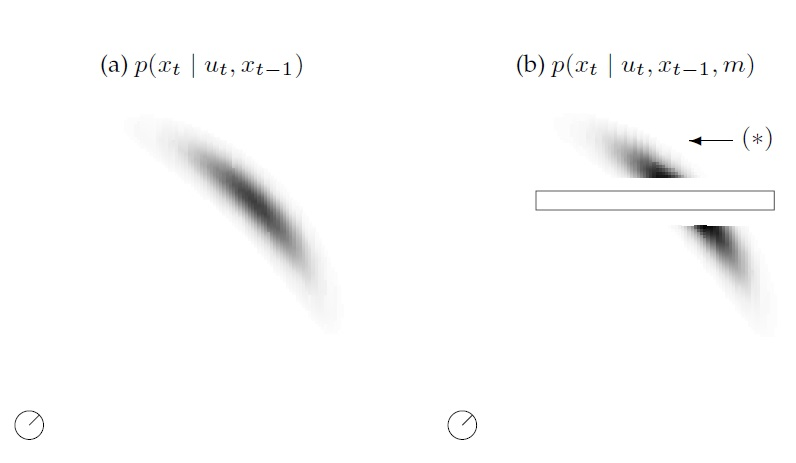
\includegraphics[width=1\linewidth]{511orig}}
	\caption{ (  Рис. 5.11 Модель движения на основе скорости (a) без карты, (b) перенесённая на карту $m$.)}
	\label{fig:511orig}
\end{figure}

На Рис. 5.11 также показана проблема такой аппроксимации. Область, отмеченная $(\ast)$, имеет ненулевое правдоподобие, поскольку и $p(x_t | u_t, x_{t-1})$ и $p(x_t | m)$ в этой области не равны нулю. Однако, чтобы робот смог попасть в эту область, он должен пройти сквозь стену, что в реальном мире невозможно. Эта ошибка является результатом проверки целостности модели только в конечном местоположении $x_t$, вместо проверки на пути к цели. На практике такие ошибки происходят только при сравнительно больших значениях $u_t$ и могут быть устранены увеличением частоты обновления.

Чтобы прояснить природу этой аппроксимации, приведём ее краткий вывод.
Выражение (5.48) можно получить из теоремы Байеса:\\

(5.49)
$$p(x_t|u_t,x_{t-1},m)=\eta\,p(m|x_t,u_t,x_{t-1})p(x_t|u_t,x_{t-1})$$
Если аппроксимировать  $p(m | x_t, u_t, x_{t-1})$ с помощью $p(m | x_t)$ и заметить, что $p(m)$ – константа, связанная в искомой апостериорной вероятностью, получим следующее искомое равенство:\\

(5.50)
\begin{equation*}
\begin{split}
p(x_t|u_t,x_{t-1},m)&=\eta\,p(m|x_t)p(x_t|u_t,x_{t-1})\\
&=\eta\,\frac{p(x_t|m)p(m)}{p(x_t)}\,p(x_t|u_t,x_{t-1})\\
&=\eta\,\frac{p(x_t|m)p(x_t|u_t,x_{t-1})}{p(x_t)}
\end{split}
\end{equation*}

Здесь $\eta$ – нормализующий член (заметим, что значение $\eta$ различно на разных этапах преобразования). Этот короткий анализ показывает, что наша модель на основе карты подтверждается при грубом допущении, что \\

(5.51)
$$p(m|x_t,u_t,x_{t-1})=p(m|x_t)$$

Очевидно, что эти выражения не равны. При вычислении условной вероятности по $m$, из аппроксимации вычёркиваются два члена: $u_t$ и $x_{t-1}$. В результате этого теряется вся информация относительно пути, ведущего к $x_t$. Все, что известно, это конечное местоположение $x_t$. Заметим, что условием вычёркивания в приведённом примере является ненулевая вероятность для робота оказаться за стеной. Если начальное и конечное местоположение находятся на свободном пространстве, приближенная модель движения на основе карты может ошибочно решить, что робот только что прошёл сквозь стену. Насколько критично это может быть? Как было замечено ранее, все зависит от величины интервала обновления. Фактически, при достаточно высоких скоростях обновления, и с учётом ограниченности переменных зашумления в модели движения, можно гарантировать, что отрицательный эффекта не возникнет, а аппроксимация останется достаточно близкой . 

В этом анализе показана одна из неочевидных особенностей реализации алгоритма -  следует обращать внимание на частоту обновления. Байесовский фильтр с очень высокой частотой обновления может показать совершенно отличный результат по сравнению с аналогичным фильтром, который обновляется лишь от случая к случаю.\\

\textbf{5.6 Вывод} \\

В этом разделе приводится вывод двух основных вероятностных моделей движения для мобильных роботов, действующих на плоскости. \\

• Был выведен  выполняемый на ограниченном интервале времени $\varDelta t$ алгоритм вероятностной модели движения $p(x_t | u_t, x_{t-1})$, выражающий параметр управления $u_t$ через поступательную и угловую скорости. При реализации модели было определено, что двух параметров шумов управления, (одного для поступательной и одного – для угловой скорости) недостаточно для генерации апостериорного распределения соответствующей размерности. В силу этого был добавлен третий параметр учёта шумов, выраженный в виде добавочного последнего действия поворота после окончания любого движения. \\

• Была представлена альтернативная модель движения, использующая одометрию робота в качестве входных данных. Измерения одометрии выражаются тремя параметрами – начальным поворотом, линейным перемещением и конечным поворотом. Вероятностная модель движения была реализована на основе зашумления всех трёх параметров. Было замечено, что показания одометра, технически говоря, не являются управляющим сигналом, однако, при использовании их в интерпретации "управления", формулировка задачи оценки сильно упростится.\\

• Для обеих моделей движения были предоставлены два типа реализаций, в одной из которых вероятность $p(x_t | u_t, x_{t-1})$ вычисляется в закрытом виде, а во втором - выполнялась генерация выборки из $p(x_t | u_t, x_{t-1})$. Выражение в закрытой форме принимает на вход $x_t$, $u_t$ и $x_{t-1}$, возвращая числовое значение вероятности. Чтобы сравнить действительные и заданные параметры управления для вычисления этой вероятности алгоритмы эффективно обращают модель движения. Модель с выборкой не требует такого обращения, поскольку в ней реализована прямая модель движения $p(x_t | u_t, x_{t-1})$. На вход принимаются значения $u_t$ и $x_{t-1}$, а на выходе находится случайный элемент $x_t$, извлечённый согласно выборке $p(x_t | u_t, x_{t-1})$. Модели в закрытом виде требуются лишь для некоторых вероятностных алгоритмов. Другие алгоритмы, в частности, многочастичные фильтры, основаны на моделях с выборкой.\\

• Наконец, все модели движения были обобщены для включения карт окружающей среды, когда в результирующей вероятности $p(x_t | u_t, x_{t-1}, m)$ учтена карту $m$. Это обобщение следует интуитивному соображению о использовании карты для определения мест, где робот может находиться, и расчёта возможности перемещения из положения $x_{t-1}$ в $x_t$. Результирующий алгоритм приведён в приближенном виде, поскольку проверяется только допустимость конечного положения.\\

Представленные модели движения являются лишь примерами. Конечно, область изучения действий роботов намного шире задачи перемещения мобильных роботов по плоской поверхности. Даже в области мобильной робототехники существует множество устройств, которые не были освещены в изложении материала. В качестве примера можно привести голономных роботов, способных двигаться в стороны без поворота или транспортные средства с подвеской. Обсуждение не включает динамику роботов, что очень важно для быстро движущихся транспортных средств, например, автомашин на шоссе. Большинство этих роботов может быть смоделировано похожим образом, для чего следует только определить физические законы движения робота и соответствующие параметры зашумления. В динамических моделях это потребует расширения состояния робота вектором скорости, который будет отображать динамическое состояние транспортного средства. По большей части, эти обобщения достаточно очевидны.  
 
Что же касается измерения собственного движения, во многих роботах для измерения движения используются инерционные датчики для дополнения или замены одометрии. Проектированию фильтров с использованием инерционных датчиков посвящены целые книги. Мы призываем читателя использовать более сложные модели и датчики в тех случаях, когда данных одометрии недостаточно.\\

\textbf{5.7 Библиографические примечания}\\

Представленный материал обобщает базовые кинематические уравнения некоторых типов мобильных роботов(Cox и Wilfong, 1990) добавлением вероятностного компонента. Используемой моделью описываются дифференциальный привод, привод Аккермана и синхронный привод (Borenstein et al., 1996). За пределами рассмотрения модели находятся приводы без неголономных ограничений (Latombe 1991), например колёсные роботы Mecanum (Ilon 1975) или шагающие роботы, наподобие описанных в перспективных работах Райберта (Raibert et al.,1986, Raibert, 1991, Saranli and Koditschek, 2002).

В робототехнике движение и взаимодействие роботов с окружающей средой изучалось весьма широко. Современные публикации по мобильной робототехнике, освещающие аспекты кинематики и динамики были написаны Мерфи (Murphy,2000c), Дудеком и Дженкином ( Dudek и Jenkin, 2000), Сигвартом и Норбакшем (Siegwart и Nourbakhsh, 2004).
Кокс и Вилфонг (Cox and Wilfong, 1990) подготовили сборник статей передовых исследователей (на момент публикации). Также можно обратиться к работе Кортенкампа (Kortenkamp et al.,1998). Классический подход к кинематике и динамике робота можно найти у Крейга (Craig, 1989), Вукобратовича (Vukobratovic, 1989), Пола (Paul, 1981) и Йошикавы (Yoshikawa, 1990).
Более современная работа по теме динамики робота была написана Физерстоуном (Featherstone, 1987). Податливое движение как одна из форм взаимодействия с окружающей средой было исследовано Мэйсоном (Mason, 2001). Механика грунтов, в части взаимодействия колёсных роботов с поверхностью была изучена в фундаментальных работах Беккера (Bekker, 1956, 1969) и Вонга (Wong, 1989). Современная публикация о взаимодействии колеса с грунтом была написана Иагнемма и Дубовски (Iagnemma and Dubowsky, 2004). Обобщение таких моделей в рамках единой вероятностной концепции – перспективное направление для будущих исследований. \\

\textbf{5.8 Упражнения}\\

1. Все модели роботов, представленные в главе - кинематические.
ДИНАМИКА
В этом упражнении будет описан робот с \textit{динамикой}. Представим робота, который находится в одномерной системе координат. Его местоположение задано координатой $x$, скорость - $\dot{x}$, ускорение - $\ddot{x}$. Допустим также, что управление влияет лишь на ускорение $\ddot{x}$. Разработать математическую модель движения, вычисляющую апостериорное положение $x'$ и скорость $\dot{x}'$ на основании начального положения $x$ и скорости $\dot{x}$. Считать, что ускорение $\ddot{x}$ является суммой указанного ускорения и гауссового шума с нулевым математическим ожиданием и дисперсией $\sigma^2$ (при условии, что ускорение в течение такта моделирования $\varDelta t$ остаётся постоянным).
Коррелируют ли $x'$ и $\dot{x}'$ в апостериорном распределении? Объяснить, почему.\\

2. Снова представим робота из упражнения 1. Написать математическую формулу вычисления апостериорного распределения по конечной скорости $\dot{x}'$, основываясь на начальном положении робота $x$, начальной скорости $\dot{x}$, и конечному положению $x'$. Что примечательного в этом распределении?\\

3. Допустим, робот управляется случайными ускорениями в течение $T$ временных интервалов, при некоем большом значении $T$. Будут ли скоррелированы конечное положение $x$ и скорость $\dot{x}$? Если да, будут ли они \textit{полностью} коррелировать при $T\uparrow\infty$, так, что одна переменная станет детерминированной функцией другой?\\

4. Представим простую кинематическую модель идеального велосипеда. Оба колеса имеют диаметр $d$, и закреплены на раме длины $l$. Переднее колесо может поворачиваться вокруг вертикальной оси, угол поворота обозначим как $\alpha$.
Заднее колесо всегда параллельно раме велосипеда и поворачиваться не может.

В этом упражнении положение велосипеда будет определено с помощью трёх переменных: координат $x-y$ центра переднего колеса, угла направления $\theta$ (поворота) рамы велосипеда по отношению к внешней системе координат. Скорость движения велосипеда вперёд $v$ и угол поворота колеса $\alpha$ будем считать постоянными в каждом такте прогнозирования.

Сформулировать математическую модель прогнозирования в интервале времени $\varDelta t$, считая, что угол поворота колеса $\alpha$  и скорость движения вперёд $v$ подвержены воздействию гауссовского шума. Модель должна прогнозировать апостериорное состояние велосипеда после промежутка времени $\varDelta t$ от известного состояния. Если точную модель найти не удаётся, сформулировать приближенную и объяснить приближения.\\

5. Вспомним кинематическую модель велосипеда из упражнения 4. Реализовать функцию выборки для апостериорных положений велосипеда при некоторых соображениях зашумленности. 
 
Для модели можно считать, что $l = 100 \text{см}, d = 80 \text{см}, \varDelta t =
1 \text{сек}, |\alpha|\leq 80^\circ, v\in [0; 100] \text{см/сек}$. Допустим, что дисперсия угла поворота колеса $\sigma_\alpha^2=25^{\circ2}$, а дисперсия скорости $\sigma_v^2=50\text {см}^2/\text{сек}^2\,\cdot\,v^2$. Заметим, что дисперсия скорости зависит от указанной скорости. 

Изобразить на графике результирующий набор элементов выборки для велосипеда, стартующего в начале координат со следующими параметрами управления:\\

\begin{table}[H]
\begin{center}
\begin{tabular}{|c|l|}
\hline
\text{problem number}&\hspace{3mm}$\alpha\hspace{13mm}v$\\
\hline
1&\hspace{2mm}$25^\circ$\hspace{7mm}$20\text{см/сек}$\\
\hline
2&\hspace{2mm}$-25^\circ$\hspace{4mm}$20\text{см/сек}$\\
\hline
3&\hspace{2mm}$25^\circ$\hspace{7mm}$90\text{см/сек}$\\
\hline
4&\hspace{2mm}$80^\circ$\hspace{7mm}$10\text{см/сек}$\\
\hline
1&\hspace{2mm}$85^\circ$\hspace{7mm}$90\text{см/сек}$\\
\hline
\end{tabular}
\end{center}
\end{table}

На всех графиках изобразить оси с единицами измерения\\

6. Снова используем модель велосипеда из упражнения 4. На основании начального состояния $x,y,\theta$ и конечных координат $x'$ и $y'$ (но без конечного угла $\theta'$), сформулировать математическую формулу для определения наиболее вероятных значений $\alpha$, $v$ и $\theta'$. Если решение в закрытом виде найти не удаётся, предложить метод аппроксимации искомых значений.\\

ГОЛОНОМНЫЙ 

7. Обычно роботы, действующие внутри помещений, оснащены какой-либо разновидностью \textit{голономного} привода. Робот с голономным приводом имеет количество управляемых степеней свободы, равное количеству измерений пространства его конфигурации (или положения). В этом упражнении требуется обобщить модель на основе скорости для голономного робота, действующего на плоскости. Условимся, что робот может управляться изменением скорости продольного и поперечного перемещения, а также скорости поворота. Произвольно будем считать положительными значения скорости поперечного перемещения, направленные влево, а отрицательными – направленные вправо. \\

• Определить математическую модель такого робота, считая что его управляющие действия подвержены независимому гауссовому шуму.\\

• Сформулировать алгоритм вычисления $p(x_t | u_t, x_{t-1})$.\\

• Сформулировать алгоритм выборки для $x_t\sim p(x_t | u_t, x_{t-1})$.\\

8. Доказать, что треугольное распределение в выражении (5.12) имеет нулевое математическое ожидание и дисперсию $b^2$. Доказать то же самое для алгоритма выборки в Таблице 5.4.\\



\end{document}